\chapter{General Relativity Lecture 2: Flatness, Tensors, and the Metric}

These notes follow Leonard Susskind's second lecture on general relativity in the order in which the ideas are introduced. The lecture begins with a methodological claim: good tensor notation should act like a set of mechanical rules, so that once the indices are placed correctly the next move is almost forced. Board captures curated by LazyingArt LLC and Video2Book are kept where they record equations or board layout that matter, but the development itself follows the spoken argument: first the intrinsic notion of flatness, then the transformation laws for tensors, and only after that the metric tensor that encodes distance.

\section{Notation, Flatness, and the Intrinsic Problem}

Susskind opens with a piece of advice that is more than advice. In tensor analysis, notation is not decoration. If the rules are good, they constrain what one is allowed to do next. The notation should behave like a set of tinker toys: a stick goes into a hole, not into another stick, and once the first move is made the next move is partly dictated. That is the spirit in which the lecture proceeds. We want enough tensor analysis, and enough control over metrics, to distinguish a genuinely flat geometry from one that only looks curved because we described it in awkward coordinates.

At first this sounds easy. Flat means plane-like; curved means bumps and lumps. But the curled page shows that this intuition is not yet sharp enough. If we take a flat sheet of paper and curl it without stretching it, the distances measured \emph{along the sheet} do not change. The embedding in the surrounding three-dimensional room changes, but the internal geometry does not. This is the distinction between extrinsic curvature and intrinsic geometry.

The lecture's little bug is the right guide. A bug confined to the surface cannot look off the surface. It can crawl, measure distances along the surface, draw triangles, and compare angles, but it has no direct access to the way the surface sits in a larger space. General relativity is interested in precisely this intrinsic geometry. The physical question is the same one we met in another language last time: is there a real gravitational field, or have we merely chosen funny spacetime coordinates?

\begin{figure}[t]
\centering
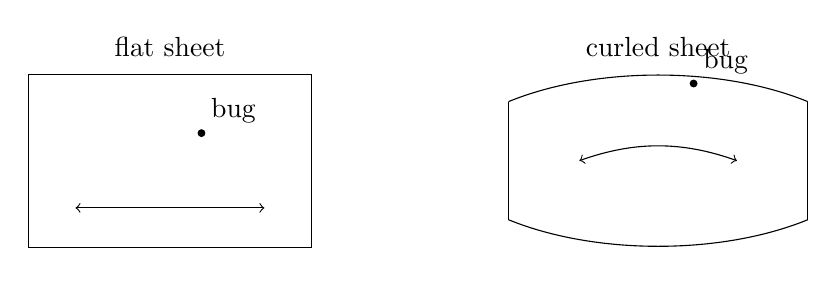
\begin{tikzpicture}[scale=1.0]
\begin{scope}
\draw (-1.8,-1.1) rectangle (1.8,1.1);
\fill (0.4,0.35) circle (0.05);
\node[above right] at (0.4,0.35) {bug};
\draw[<->] (-1.2,-0.6) -- (1.2,-0.6);
\node at (0,1.45) {flat sheet};
\end{scope}

\begin{scope}[xshift=6.2cm]
\draw (-1.9,0.75) .. controls (-0.8,1.2) and (0.8,1.2) .. (1.9,0.75);
\draw (-1.9,-0.75) .. controls (-0.8,-1.2) and (0.8,-1.2) .. (1.9,-0.75);
\draw (-1.9,0.75) -- (-1.9,-0.75);
\draw (1.9,0.75) -- (1.9,-0.75);
\fill (0.45,0.98) circle (0.05);
\node[above right] at (0.45,0.98) {bug};
\draw[<->] (-1.0,0.0) .. controls (-0.3,0.25) and (0.3,0.25) .. (1.0,0.0);
\node at (0,1.45) {curled sheet};
\end{scope}
\end{tikzpicture}
\caption{Schematic reconstruction of the curled-page argument. The embedding changes, but lengths measured along the page do not. The bug, confined to the surface, has access only to the intrinsic geometry.}
\end{figure}

This gives the lecture its first real pivot. The problem of flatness is not merely a visual problem. It is a problem about the internal relations among nearby points. That same problem, translated into spacetime language, becomes the question of whether we are seeing real gravity or merely a misleading coordinate description.

\subsection{Question \& Answer}

The natural question comes immediately: what does \emph{flat} mean?

At this point the lecture gives only a preview, not the full machinery. The intuitive answer is that a flat space can be laid out without distortion. But the mathematical answer, the one we will eventually earn, is stated in terms of the metric tensor: in a flat space one can choose coordinates so that the metric becomes the Kronecker delta,
\begin{equation}
g_{mn}=\delta_{mn},
\end{equation}
for the ordinary positive-definite geometry being discussed here. That is the target, but we are not yet entitled to use it until we know what a tensor is and how a metric transforms.

Before we can answer the question in earnest, we need the language that will let us even state it properly.

\section{Triangulations and the Intuition for Curvature}

The lecture now makes the intrinsic viewpoint operational. Imagine sprinkling points through the space, joining neighboring points by links, and specifying the lengths of those links. In this way the geometry is encoded by neighboring distances. If those distances can be realized in a flat layout without changing any link length, then the geometry is flat. If they cannot, then the curvature is intrinsic.

A triangular lattice is the cleanest example. If the links form equilateral triangles, and the joints are free to hinge, the whole structure can still be laid flat on the desk. Nothing in those local distances forces a bulge. But if we enlarge the six links that meet a single node, that node is forced out of the plane. A bulge appears, and it cannot be pressed back into the plane without altering the lengths of the links. That is the lecture's concrete model of curvature.

\begin{figure}[t]
\centering
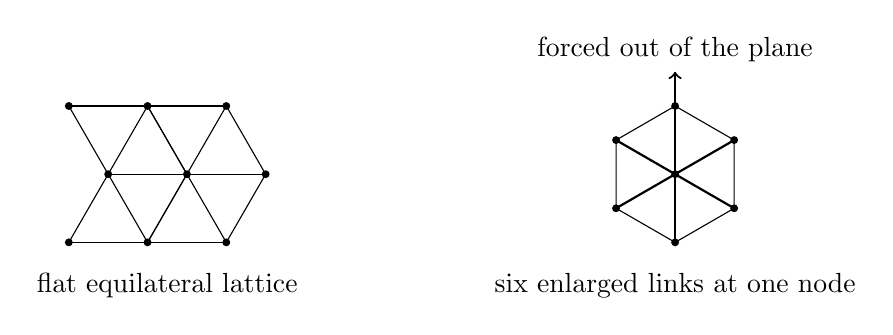
\begin{tikzpicture}[scale=1.0]
\begin{scope}
\draw (0,0) -- (1,0) -- (2,0);
\draw (0.5,0.866) -- (1.5,0.866) -- (2.5,0.866);
\draw (0,1.732) -- (1,1.732) -- (2,1.732);
\draw (0,0) -- (0.5,0.866) -- (0,1.732);
\draw (1,0) -- (1.5,0.866) -- (1,1.732);
\draw (2,0) -- (2.5,0.866) -- (2,1.732);
\draw (0.5,0.866) -- (1,0) -- (1.5,0.866) -- (2,0);
\draw (0.5,0.866) -- (1,1.732) -- (1.5,0.866) -- (2,1.732);
\foreach \x/\y in {0/0,1/0,2/0,0.5/0.866,1.5/0.866,2.5/0.866,0/1.732,1/1.732,2/1.732}
  \fill (\x,\y) circle (0.05);
\node at (1.25,-0.55) {flat equilateral lattice};
\end{scope}

\begin{scope}[xshift=6.7cm]
\coordinate (O) at (1,0.866);
\coordinate (A) at (1,1.732);
\coordinate (B) at (1.75,1.299);
\coordinate (C) at (1.75,0.433);
\coordinate (D) at (1,0);
\coordinate (E) at (0.25,0.433);
\coordinate (F) at (0.25,1.299);

\draw (A) -- (B) -- (C) -- (D) -- (E) -- (F) -- (A);
\draw[thick] (O) -- (A);
\draw[thick] (O) -- (B);
\draw[thick] (O) -- (C);
\draw[thick] (O) -- (D);
\draw[thick] (O) -- (E);
\draw[thick] (O) -- (F);
\draw[->,thick] (O) -- ++(0,1.3) node[above] {forced out of the plane};

\foreach \p in {O,A,B,C,D,E,F}
  \fill (\p) circle (0.05);

\node at (1.0,-0.55) {six enlarged links at one node};
\end{scope}
\end{tikzpicture}
\caption{Schematic reconstruction of the triangulation argument. Equal neighboring distances can be realized in a flat layout; altering the six links that meet one node forces a bulge if the lengths are to remain fixed.}
\end{figure}

This is the lecture's first real criterion in geometric language. A curved space is not merely one that can be bent in a higher-dimensional room. It is one that cannot be flattened without changing the distances that define it. That is why the distinction is intrinsic rather than extrinsic.

So the question becomes sharper. If we are given a geometry in coordinates, what object are we usually given? The answer, Susskind says, is the metric tensor. But before we can use it, we need a more systematic discussion of tensors themselves.

\section{Coordinates, Basis Vectors, and Two Kinds of Components}

Before turning to abstract transformation laws, the lecture pauses for a geometric interlude. This is not yet the official definition of tensors. It is a way of seeing why upper and lower indices must be treated differently outside Cartesian coordinates.

Take coordinates \(x^1,x^2,\dots\) that need not be perpendicular, and need not be spaced in physical units. A change of one coordinate unit along the \(m\)-th direction defines a basis vector \(E_m\). These basis vectors are not assumed to be orthogonal, and their lengths need not be one.

Now take an arbitrary vector \(V\). We can expand it in the basis:
\begin{equation}
V = V^m E_m.
\end{equation}
The coefficients \(V^m\) are numbers, not vectors. They tell us how much of each basis vector is needed to build \(V\). These are the contravariant components. They are, in Susskind's phrase, the expansion coefficients.

The covariant components are defined differently. They are the dot products of \(V\) with the basis vectors:
\begin{equation}
V_n = V \cdot E_n.
\end{equation}
Substituting the expansion of \(V\), we find
\begin{equation}
V_n = V^m(E_m\cdot E_n).
\end{equation}
This isolates a new object,
\begin{equation}
g_{mn}=E_m\cdot E_n,
\end{equation}
which is precisely the metric tensor in this basis picture. Therefore
\begin{equation}
V_n=g_{mn}V^m.
\end{equation}
The two kinds of components coincide only in the special case of orthonormal Cartesian coordinates.

The same construction gives the length of the vector:
\begin{equation}
V\cdot V=(V^mE_m)\cdot(V^nE_n)=g_{mn}V^mV^n.
\end{equation}
This is the first appearance of the metric in the lecture as the object that computes squared length.

\begin{figure}[t]
\centering
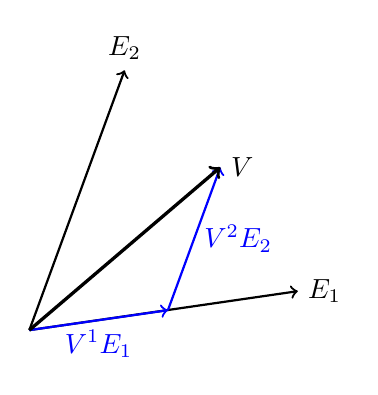
\begin{tikzpicture}[scale=1.1]
\draw[->,thick] (0,0) -- (3.1,0.45) node[right] {$E_1$};
\draw[->,thick] (0,0) -- (1.1,3.0) node[above] {$E_2$};

\draw[->,blue,thick] (0,0) -- (1.6,0.23) node[midway,below] {$V^1E_1$};
\draw[->,blue,thick] (1.6,0.23) -- (2.205,1.88) node[midway,right] {$V^2E_2$};

\draw[->,very thick] (0,0) -- (2.205,1.88) node[right] {$V$};
\end{tikzpicture}
\caption{Schematic reconstruction of oblique coordinates. The contravariant components are the coefficients in the expansion \(V=V^mE_m\), while the covariant components arise from dot products with the basis vectors.}
\end{figure}

A subtle point is worth preserving from the lecture. Before the metric is introduced abstractly, contravariant vectors and covariant vectors are to be treated as different kinds of objects. The basis-vector picture hints at a correspondence between them through \(V_n=g_{mn}V^m\), but the lecture does not yet want us to identify them wholesale. That identification will become systematic only once the metric has been defined on its own terms.

The lecture then sharpens the geometric picture one more time. Orthogonality by itself is not enough to recover Cartesian simplicity. Polar coordinates are orthogonal, but the separation corresponding to a fixed angular increment grows with radius. So even when coordinate directions meet at right angles, the basis vectors need not behave as they do in Cartesian coordinates.

\begin{figure}[t]
\centering
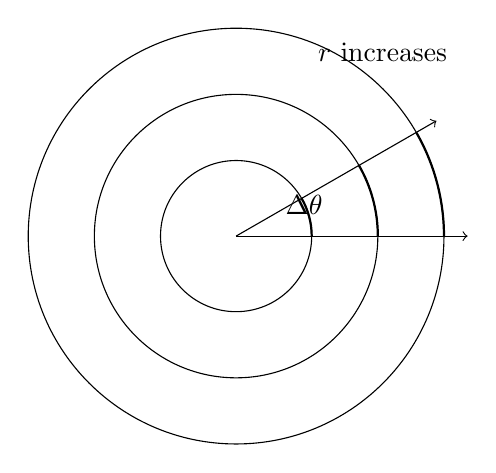
\begin{tikzpicture}[scale=1.2]
\draw (0,0) circle (0.8);
\draw (0,0) circle (1.5);
\draw (0,0) circle (2.2);
\draw[->] (0,0) -- (2.45,0);
\draw[->] (0,0) -- (2.12,1.22);
\draw[thick] (0.8,0) arc[start angle=0,end angle=30,radius=0.8];
\draw[thick] (1.5,0) arc[start angle=0,end angle=30,radius=1.5];
\draw[thick] (2.2,0) arc[start angle=0,end angle=30,radius=2.2];
\node at (0.72,0.33) {$\Delta\theta$};
\node at (1.55,1.95) {$r$ increases};
\end{tikzpicture}
\caption{Schematic reconstruction of the polar-coordinate refinement. The coordinate directions are orthogonal, but the physical separation associated with a fixed angular increment grows with radius. Orthogonality alone does not make a coordinate system Cartesian.}
\end{figure}

Only after this detour does Susskind say, in effect, now let us come to tensor analysis proper.

\section{Tensors by Their Transformation Laws}

For a while we are asked to proceed in the safest possible way: not by leaning on geometric pictures, but by letting the transformation law define the object. A tensor, at least at first, is whatever transforms in the right way.

Let \(x^m\) and \(y^m\) be two coordinate systems on the same space, related by an invertible differentiable change of variables. We will mostly be interested in tensor \emph{fields}: a different tensor attached to each point of space, varying from point to point. Prime notation will refer to components written in the \(y\)-coordinates, and unprimed notation to components written in the \(x\)-coordinates.

The simplest tensor is a scalar field \(S\). Everybody agrees on its value at a given point, so
\begin{equation}
S'(y)=S(x).
\end{equation}

A contravariant vector transforms like a little coordinate displacement:
\begin{align}
V'^m &= \frac{\partial y^m}{\partial x^n}V^n, \\
dy^m &= \frac{\partial y^m}{\partial x^n}dx^n.
\end{align}
The differential \(dx^m\) is the archetype. Its components transform with the Jacobian \(\partial y/\partial x\), and that is exactly what a contravariant vector does.

A covariant vector transforms the other way:
\begin{equation}
W'_m=\frac{\partial x^n}{\partial y^m}W_n.
\end{equation}
The gradient of a scalar is the standard example:
\begin{equation}
\frac{\partial S}{\partial y^m}
=
\frac{\partial x^n}{\partial y^m}\frac{\partial S}{\partial x^n}.
\end{equation}
This is nothing but the chain rule, written in tensor notation. Since there are several coordinates, these derivatives are partial derivatives throughout.

The general pattern is systematic. Each upper \(y\)-index contributes a factor of \(\partial y/\partial x\), and each lower \(y\)-index contributes a factor of \(\partial x/\partial y\). Thus a mixed rank-two tensor transforms as
\begin{equation}
T'^m{}_n
=
\frac{\partial y^m}{\partial x^p}
\frac{\partial x^q}{\partial y^n}
T^p{}_q,
\end{equation}
while a purely covariant rank-two tensor transforms as
\begin{equation}
W'_{mn}
=
\frac{\partial x^p}{\partial y^m}
\frac{\partial x^q}{\partial y^n}
W_{pq}.
\end{equation}

This is where the opening claim about notation begins to pay off. The indices do not merely label components. They tell us what sort of Jacobian factors are allowed to appear, and they keep track of which contractions are legal. One begins to see what Susskind means when he says that good notation carries you along.

\section{Tensor Equations, Tensor Products, and Contraction}

Once tensors are defined by their transformation laws, their main use becomes visible at once: tensor equations have the same truth value in every coordinate system, provided the two sides have the same index structure.

\begin{proposition}
If all components of a tensor vanish in one coordinate system, then all components vanish in every coordinate system.
\end{proposition}

\begin{proof}
Each transformed component is a linear combination of the original components. Therefore zero maps to zero.
\end{proof}

\paragraph{What is invariant?}
Not the individual components; they change from frame to frame. What is invariant is the truth of the tensor equation. If \(W=T\) for two tensors of the same type, then \(W-T=0\) in one coordinate system, and therefore in every coordinate system. But if the index structure fails to match, the equation has no coordinate-independent meaning. This is exactly the point the lecture insists on when it refuses to equate unlike tensors.

The subtraction rule makes this concrete. If \(T\) and \(S\) are tensors of the same type, then
\begin{equation}
T^{m\cdots}{}_{\cdots p}-S^{m\cdots}{}_{\cdots p}
=
(T-S)^{m\cdots}{}_{\cdots p}.
\end{equation}
The ellipses are deliberate: the board suppresses the full rank, and we should not invent it. What matters is that the index pattern matches on both sides. Then \(T-S=0\) is a tensor equation, and if it is true in one frame it is true in every frame.

\begin{figure}[t]
\centering

\includegraphics[width=0.78\textwidth]{lecture_02_figure_02.png}
\caption{Tensor subtraction as a tensor equation. The board keeps the suppressed indices generic, but the mathematical point is complete: the difference of two tensors of the same type is another tensor of that same type.}
\end{figure}

Tensor multiplication, by contrast, raises rank rather than preserving it. If \(V^m\) is contravariant and \(W_n\) is covariant, then
\begin{equation}
T^m{}_n = V^mW_n
\end{equation}
is a rank-two tensor. This is the tensor product, or outer product. It is \emph{not} the dot product. In four dimensions it has sixteen components, not one. The components commute as numbers, but the order of the tensor slots still matters: the first index belongs to one factor, the second to the other.

Contraction is the next operation, and here the lecture pauses for a lemma.

\begin{proposition}
For any invertible coordinate transformation \(x \leftrightarrow y\),
\begin{equation}
\frac{\partial x^b}{\partial y^m}\frac{\partial y^m}{\partial x^a}
=
\delta^b{}_a.
\end{equation}
\end{proposition}

\begin{proof}
For any differentiable function \(f\),
\begin{equation}
\frac{\partial f}{\partial y^m}\frac{\partial y^m}{\partial x^a}
=
\frac{\partial f}{\partial x^a}
\end{equation}
by the chain rule. Choosing \(f=x^b\), we obtain
\begin{equation}
\frac{\partial x^b}{\partial y^m}\frac{\partial y^m}{\partial x^a}
=
\frac{\partial x^b}{\partial x^a}
=
\delta^b{}_a.
\end{equation}
\end{proof}

Now let
\begin{equation}
T^m{}_n=V^mW_n.
\end{equation}
Its transformation law is
\begin{equation}
T'^m{}_n
=
\frac{\partial y^m}{\partial x^a}
\frac{\partial x^b}{\partial y^n}
V^aW_b.
\end{equation}
If we contract the upper and lower indices, we obtain
\begin{align}
T'^m{}_m
&=
\frac{\partial y^m}{\partial x^a}
\frac{\partial x^b}{\partial y^m}
V^aW_b \\
&=
\delta^b{}_a\,V^aW_b \\
&=
V^aW_a.
\end{align}
The contraction \(V^mW_m\) has no free indices and has the same value in every coordinate system. It is therefore a scalar.

This is the lecture's tensor-algebra version of the inner product. More generally, when we contract one upper index with one lower index, the rank drops by two.

\subsection{Question \& Answer}

Why may we contract only an upper index with a lower one?

Because only then do the Jacobians collapse to a Kronecker delta. If we start instead with a tensor carrying two upper indices, for example \(U^{mn}\), then its transformation law contains two factors of \(\partial y/\partial x\):
\begin{equation}
U'^{mn}
=
\frac{\partial y^m}{\partial x^a}
\frac{\partial y^n}{\partial x^b}
U^{ab}.
\end{equation}
If one now tries to identify the two upper indices, the Jacobian factor becomes
\begin{equation}
\frac{\partial y^m}{\partial x^a}
\frac{\partial y^m}{\partial x^b},
\end{equation}
and this is not the mixed product that yields \(\delta^b{}_a\). Nothing simplifies. One does not get a tensor. So the notation is not merely etiquette here; it enforces what operations are legal.

The lecture briefly lists one more tensor operation, covariant differentiation, but does not develop it yet. That is postponed. The real mathematical payoff of the present lecture comes next, when we return to the metric tensor that was deferred at the beginning.

\section{The Metric Tensor as the Quadratic Form of Distance}

Only now, after the detour through tensor algebra, do we come back to the central object. Susskind first reminds us that the basis-vector construction already produced a metric through \(E_m\cdot E_n\). But he now wants the metric tensor defined on its own terms, abstractly.

Consider a little displacement vector with contravariant components \(dx^m\). Its squared length is defined by the metric tensor:
\begin{equation}
ds^2 = g_{mn}(x)\,dx^m dx^n.
\end{equation}
This is the cautious canonical way to typeset what the lecture repeatedly calls ``the squared length of the little \(dx\) vector.''

Several points are already built into this formula. First, the metric can depend on position. Second, the expression is quadratic in the coordinate differentials. Third, in general coordinates the analogue of the Pythagorean theorem is still quadratic, but no longer diagonal.

The lecture then asks how many independent components the metric has. In four dimensions there are initially \(4\times 4=16\) coefficients. But since \(dx^m dx^n = dx^n dx^m\), there is no need to distinguish \(g_{12}\) from \(g_{21}\), and similarly for every off-diagonal pair. That reduces the count to \(10\). In three dimensions the count is \(6\), and in two dimensions it is \(3\):
\begin{equation}
16 \longrightarrow 10, \qquad 9 \longrightarrow 6, \qquad 4 \longrightarrow 3.
\end{equation}

What still needs proof is that \(g_{mn}\) really is a tensor. The guiding principle is that length is a scalar. Everyone may disagree about the components of a vector, but everyone agrees about its squared length. Therefore
\begin{equation}
g_{mn}(x)\,dx^m dx^n
=
g'_{pq}(y)\,dy^p dy^q.
\end{equation}
Now rewrite the differentials in terms of the primed coordinates:
\begin{equation}
dx^m=\frac{\partial x^m}{\partial y^p}\,dy^p,
\qquad
dx^n=\frac{\partial x^n}{\partial y^q}\,dy^q.
\end{equation}
Substituting these into the unprimed expression gives
\begin{align}
ds^2
&=
g_{mn}(x)
\left(\frac{\partial x^m}{\partial y^p}dy^p\right)
\left(\frac{\partial x^n}{\partial y^q}dy^q\right) \\
&=
g_{mn}(x)\,
\frac{\partial x^m}{\partial y^p}
\frac{\partial x^n}{\partial y^q}
\,dy^pdy^q.
\end{align}
Comparing with \(ds^2=g'_{pq}(y)\,dy^pdy^q\), we identify the coefficient of \(dy^pdy^q\) as the primed metric:
\begin{equation}
g'_{pq}(y)
=
g_{mn}(x)\,
\frac{\partial x^m}{\partial y^p}
\frac{\partial x^n}{\partial y^q}.
\end{equation}
This is exactly the transformation law of a covariant rank-two tensor.

\begin{figure}[t]
\centering

\includegraphics[width=0.88\textwidth]{lecture_02_figure_03.png}
\caption{Metric tensor in primed and unprimed coordinates. The board isolates \(g'_{pq}(y)\) in a small box and the transformed coefficient built from \(g_{mn}(x)\) and two Jacobians in a larger box; the lecture's point is that these must be the same object.}
\end{figure}

The board capture is helpful here. The auxiliary substitution lines for \(dx^m\) and \(dx^n\) are only partially visible, so we typeset them in their standard canonical form. But the important visual evidence is fully present: the small box around \(g'_{pq}(y)\) and the large box around the transformed coefficient tell us exactly which object is to be read as the metric in the new coordinates.

This also explains why the metric carries two lower indices: it multiplies two contravariant displacement components \(dx^m\) and \(dx^n\). In this way the lecture returns cleanly to the question it postponed. If flatness is to be decided from the metric, then we must first know that the metric is genuinely a tensor.

\section{The Metric as a Symmetric Matrix and Its Inverse}

At this stage the lecture changes point of view. The metric tensor is not only a tensor; it is also a matrix. Since \(dx^m dx^n = dx^n dx^m\), we may take
\begin{equation}
g_{mn}=g_{nm}.
\end{equation}
In other words, the metric is a symmetric matrix. This symmetry should be derived from the quadratic form itself, not from the somewhat garbled late discussion on the board.

For the ordinary Riemannian geometry being discussed in this lecture, Susskind then assumes that the metric has no zero eigenvalues. The matrix is therefore invertible. He denotes its inverse by \(g^{mn}\), the metric with upstairs indices, and writes the inverse relation as
\begin{equation}
g_{mn}g^{np}=\delta_m{}^p.
\end{equation}
This is the index notation for the statement that a matrix multiplied by its inverse gives the identity matrix.

\paragraph{Where do these tensors live?}
A late student question asks what space these vectors and tensors live in. The useful answer is the tangent space. At each point of the curved space there is a tangent space of the same dimension, and vectors and higher tensors at that point are naturally regarded as living there. This is why the index ranges match the dimension of the underlying space.

\subsection{Question \& Answer}

In what sense is \(g_{mn}g^{np}=\delta_m{}^p\) the identity matrix?

The right way to read the formula is that \emph{the whole array} of quantities with row index \(m\) and column index \(p\) is the identity matrix. One does \emph{not} mean that only the case \(m=p\) is being discussed. Rather, for every pair \((m,p)\) there is one equation, and together those equations form the statement that the product matrix is the identity.

The Kronecker delta is the mixed-index identity tensor:
\begin{equation}
\delta_m{}^p
=
\begin{cases}
1, & m=p,\\
0, & m\neq p.
\end{cases}
\end{equation}
So the matrix equation simultaneously contains the diagonal equations that give \(1\) and the off-diagonal equations that give \(0\).

In two dimensions the lecture writes this out as
\begin{equation}
\begin{pmatrix}
g_{11} & g_{12} \\
g_{21} & g_{22}
\end{pmatrix}
\begin{pmatrix}
g^{11} & g^{12} \\
g^{21} & g^{22}
\end{pmatrix}
=
\begin{pmatrix}
1 & 0 \\
0 & 1
\end{pmatrix}.
\end{equation}
Since the metric is symmetric, we also have \(g_{21}=g_{12}\). Reading off the entries gives four scalar equations. Two of them are
\begin{align}
g_{11}g^{11}+g_{12}g^{21} &= 1, \\
g_{11}g^{12}+g_{12}g^{22} &= 0,
\end{align}
and two more come from the second row. This is the precise meaning of the identity-matrix statement.

\begin{figure}[t]
\centering

\includegraphics[width=0.88\textwidth]{lecture_02_figure_06.png}
\caption{Inverse metric identity and symmetric matrix example. The board ties together the transformed line element, the inverse-metric relation, and the explicit \(2\times 2\) matrix picture.}
\end{figure}

The board frame is especially useful here because it preserves the lecture's sequencing: the transformed line element remains across the top, the inverse-metric identity sits at left, and the small \(2\times 2\) matrix example appears below. The matrix product on the board is unfinished, so the clean LaTeX rewrite above should be taken as a cautious completion of what the lecture is visibly setting up.

The lecture then adds an important caveat. In an ordinary geometry where squared lengths are positive, the metric is positive definite. But this is not how spacetime geometry will finally work. In relativity one encounters signatures such as
\begin{equation}
ds^2=t^2-x^2-y^2-z^2
\end{equation}
or the opposite sign convention. So the later Lorentzian metric will not be positive definite. Even so, the matrix can remain invertible; null vectors do not imply zero eigenvalues. This caveat matters because the lecture's claim about nonzero eigenvalues belongs only to the ordinary positive-metric discussion of tonight's lecture.

\section{Summary}

The lecture has now earned the preview it gave near the beginning. Flatness will ultimately be a statement about the metric, but one must first understand what tensors are, how their indices transform, and what operations preserve tensor character. We began with the intrinsic geometry of a curled page and a triangulated lattice, moved through contravariant and covariant components, built tensor equations, tensor products, and contractions, and returned at last to the metric tensor as the quadratic form of distance.

This is also exactly where the lecture stops. So far, as Susskind says, the material is mostly the discipline of notation and the algebra it permits. The next step is differentiation. If the question of flatness is to be answered in earnest, we must know how the metric varies from point to point. That means covariant differentiation, and then curvature.